\documentclass{article}
\usepackage[utf8]{inputenc}
\usepackage{wasysym}
\usepackage{qrcode}
\usepackage[colorlinks]{hyperref}
\usepackage{lmodern}
\usepackage{graphicx}
\usepackage{xcolor}
\usepackage[left=2cm, top=3cm, right=2cm]{geometry}
\usepackage{booktabs}
\usepackage{svg}
\usepackage{minted}
\usepackage{xcolor}
\definecolor{LightGray}{gray}{0.975}

%setup new colors
\hypersetup{
%linkcolor=blue
%,citecolor=
%,filecolor=
urlcolor=blue
%,menucolor=
%,runcolor=
%,linkbordercolor=
%,citebordercolor=
%,filebordercolor=
%,urlbordercolor=
%,menubordercolor=
%,runbordercolor=
}

\title{Databases \\ Lab 06: ERD.}
\author{Andrés Calderón, Ph.D.}
\date{\today}

\begin{document}

\maketitle

\section{Introduction}

In modern software systems, data is at the core of nearly every application —and designing a solid data structure from the beginning is crucial. The Entity-Relationship Diagram (ERD) is a powerful conceptual tool that allows developers, analysts, and database architects to visually map the structure and relationships within a database before it's built.

In this lab, you will explore the fundamentals of the ER model, learning how to identify key components such as entities, relationships, attributes, and cardinalities. You'll also gain hands-on experience in designing an ERD based on real-world scenarios, setting the foundation for creating robust and scalable relational databases. This tutorial draws inspiration from the article \textit{``Entity-Relationship Model of a Database: What It Is, Elements, and Examples''} by iLerna\footnote{Available at \url{https://www.ilerna.es/blog/modelo-entidad-relacion-base-datos}}, providing a clear and practical guide for understanding and applying ER modeling techniques.

\section{What is the Entity-Relationship Model?}

The entity-relationship model, entity-relationship diagram, or ERD, is a tool used in the second phase of database design.

This diagram, created by computer scientist Peter Chen, visually and simplistically represents how people, objects, or concepts within a system are connected.

The ER model allows organizing and visualizing the information structure before creating the final database, providing a clear and easy-to-understand schema for designing how data will be stored and related.

\section{Elements of the Entity-Relationship Model}

The ER diagram consists of four basic elements:

\begin{itemize}
    \item Entities
    \item Relationships
    \item Attributes
    \item Cardinalities
\end{itemize}

\begin{figure}
	\centering
	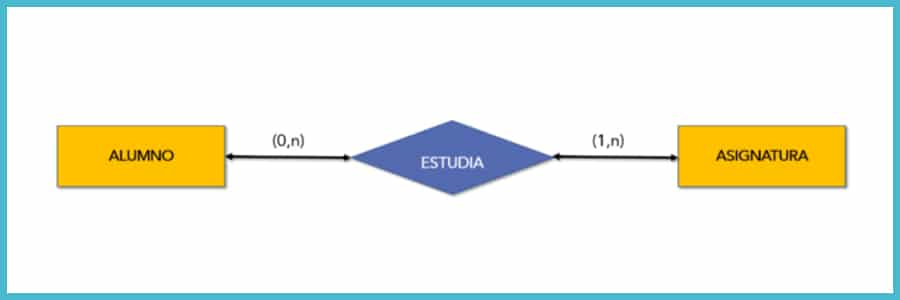
\includegraphics[bb=0 0 900 300, width=0.5\textwidth]{figures/entidad-relacion-ejemplo.jpg}
	\label{fig:erexample1}
	\caption{Simple schema of a relationship between two entities and their cardinalities.}
\end{figure}

\subsection{Entity}

Entity sets are elements about which information is collected to represent in the database. There are two types of entities, represented graphically with a rectangle:

\begin{itemize}
    \item \textbf{Strong entities}: Do not depend on other entities to exist. For example, a student in a school's database is a strong entity because they exist independently.
    \item \textbf{Weak entities}: Depend on a strong entity to make sense. For instance, an order in an online store is a weak entity because it is always linked to a customer.
\end{itemize}

\subsection{Relationship}

A relationship indicates how two or more entities interact or connect. It is represented with a diamond and is usually expressed as a verb. There are different types of relationships according to their degree:

\begin{itemize}
    \item \textbf{Degree 1 or unary relationship}: Relates an entity to itself. For example, a class delegate who is also a student of the course.
    \item \textbf{Degree 2 or binary relationship}: Connects two different entities. For example, a supplier that provides items.
    \item \textbf{Degree 3 or ternary relationship}: Links three or more entities. For example, a bank customer who has several accounts, each in a different branch.
\end{itemize}

Relationships between entities can have different types of correspondence, indicating how they connect:

\begin{itemize}
    \item \textbf{1:1 (One to one)}: Each element of the first entity corresponds to one and only one of the second entity, and vice versa. For example, a hotel guest occupies a single room, or a class of students is assigned to a single classroom, and only that group attends that classroom.
    \item \textbf{1:N (One to many)}: Each element of the first entity corresponds to one or more elements of the second entity, but each element of the second entity corresponds to only one of the first entity. An example would be a supplier that provides several items, but each item has a single supplier.
    \item \textbf{N:M (Many to many)}: Several occurrences of one entity can be associated with several of the other. For example, a student can enroll in several courses, and each course can have several enrolled students.
\end{itemize}

\subsection{Attributes}

Attributes are the characteristics or details that describe an entity. They are like the properties that define an element within existing databases.

For example, if we have an entity called Person, some of its attributes could be:

\begin{itemize}
    \item Name
    \item Age
    \item ID (which would be unique for each person)
\end{itemize}

The set of attributes helps provide more information about an entity, such as a student's name or a customer's date of birth. In a diagram, attributes are represented with circles.

\subsection{Cardinality}

Cardinality defines how many times an entity can be related to another. Basically, it shows how many elements of one entity can be associated with those of another entity.

For example, in a 1:1 relationship, like a car and its license plate, each car has only one license plate, and each license plate belongs to a single car. In a 1:N relationship, like a customer and their orders, a customer can place several orders, but each order belongs to only one customer.

In an N:M relationship, like that of students and courses, several students can be enrolled in several courses, and each course can have several students.

\section{How to Design a Conceptual Database Schema}

The conceptual schema of a database provides an overview of how data will be organized and what relationships will exist between them. It is the first step to correctly structure the database, and the steps to follow to design it are as follows.

\subsection{Gather Client Information}

It is essential to gather all the necessary information from the client to understand their needs. This allows designing a database that truly meets the user's requirements and aligns with their objectives.

\subsection{Design the Entity-Relationship Model}

In this step, the entity-relationship (ER) diagram is created, incorporating the collected data. Standard graphical rules are followed: entities are represented with rectangles, relationships with diamonds, and attributes with circles.

This model helps visualize how the different elements within the database are connected.

\subsection{Create the Relational Model}

Once we have the conceptual diagram, it is transformed into a relational model. In this stage, entities and relationships are organized into tables containing the data, and the relationships between them are defined. This facilitates implementation in a real system.

\subsection{Decide on the Database Management System (DBMS)}

With the model clear, it is necessary to choose the Database Management System (DBMS) that best suits the project's needs. This system is the software that will allow creating, managing, and querying the database.

\subsection{Implement the Model in the Program}

Finally, the relational model must be implemented in the selected DBMS. In this phase, the conceptual model becomes a physical data model that will be managed by the system, and the data will be ready to be used in the application.

\section{Examples of Entity-Relationship}

Below is an example of how a database would be graphically represented with the following entities: author, book, copy, and user:

\begin{itemize}
    \item \textbf{Author}: The attributes of the author entity are code and name. The code is the main attribute, as it is unique for each author.
    \item \textbf{Book}: The attributes of the book entity are pages, code, title, ISBN, and publisher. The code is the main attribute and is unique for each book.
    \item \textbf{Copy}: The attributes of the copy entity are code and location. The code is the main attribute and is unique for each copy.
    \item \textbf{User}: The attributes of the user entity are code, name, phone number, and address. The code is the main attribute and is unique for each user.
\end{itemize}

In this model, there are three main relationships:

\begin{itemize}
    \item \textbf{Author - Book}: An author can write several books. This is a relationship between the \texttt{author} and \texttt{book} entities.

    \item \textbf{Book - Copy}: A book can have multiple copies. This relationship connects the \texttt{book} and \texttt{copy} entities.

    \item \textbf{User - Copy}: A user can have several borrowed copies. This is the relationship between the \texttt{user} and \texttt{copy} entities.
\end{itemize}

\begin{figure}
	\centering
	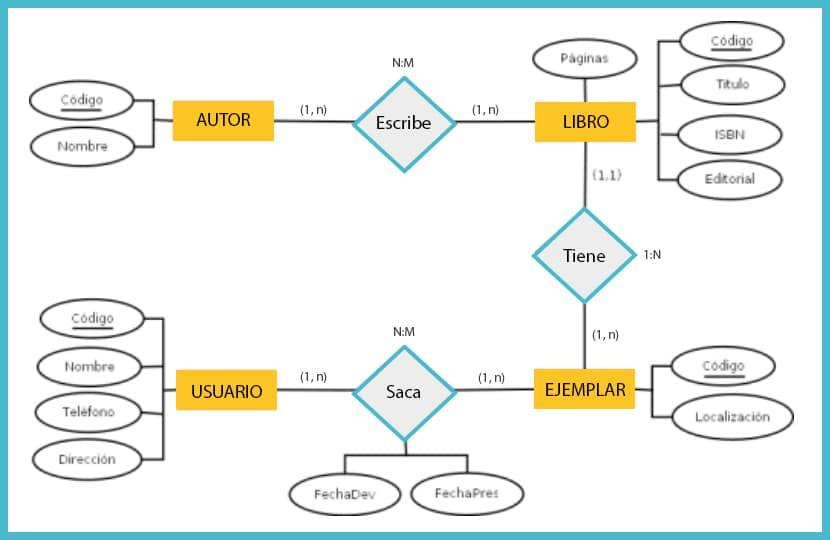
\includegraphics[width=0.6\textwidth]{figures/entidad-relacion-ejemplo2.jpg}
	\label{fig:erexample2}
	\caption{Example of a representation of a Entity-Relationship model.}
\end{figure}

\section{Independent Work}
You will read the following \href{https://drive.google.com/file/d/1TOvNSZZsybj1skLCpOxLtpr8b5A3Zb_6/view?usp=sharing}{exercises} and choose \textbf{one} of them. You will then create your first attempt at an E-R model by identifying the main entities, relationships, attributes, and cardinalities, following a similar approach to the previous example. For now, draw your diagram by hand, scan it, and include it in a well-organized report where you discuss the main aspects of your analysis and design decisions.

Please (PLEASE!) submit your report in \textbf{PDF format} by email with the subject {\LARGE \texttt{\textbf{[DBS] Lab 07}}} no later than \textbf{April 10, 2025}.

\vspace{5mm}
Happy Hacking! \includesvg[width=4mm]{figures/sunglasses}

\end{document}

